\subsection{General}
\subsubsection{Online TikZ manuel}
\url{https://tikz.dev/}\\
\subsubsection{Package and libraries}
\verb|\usepackage{tikz}| using tikz package\\
\verb|\usetikzlibrary{positioning}| Load a given tikz library\\
\subsubsection{Syntax}
\verb|\coordinate (X) at (3,5);| name a point X\\
\verb|\node[options] (X) at (3,5) {};| place a node and name it X\\

\subsection{Coordinate specifications}
\subsubsection{Coordinate calculations}
\begin{tabular}[]{p{0.1\textwidth}p{0.1\textwidth}l}
&&library needed\\
$(x,y)$&Cartesian coordinates&\\
($\theta$:r)&polar coordinates&\\
\verb |($(A)+{sin(60)}*(B)$)|         &coordinate calculations&calc\\
\verb |($(A)!.25!(B)$)|&                 partway calculations&calc\\
\verb |($(A)!3cm!(B)$)|&                 3~cm from (A) in direction of (B)&calc\\
\verb |($(A)!1.2!30:(B)$)|&              stretch by 1.2, then rotate by 30$^{\circ}$&calc\\
\verb |($(A)!(B)!(C)$)|&                 projection of point B onto line AC&calc\\
\verb |($(A)!(B)!30:(C)$)|&              project B onto line AC, then rotate by 30$^{\circ}$&calc\\
\verb '(n1-|n2)'& projection of n2 on the line passing through n1\\
\verb '(n1|-n2)'& projection of n1 on the line passing through n2\\
\verb |\node[above=1cm of| \verb|somenode.north]|&position new node 1~cm above existing anchor&positioning\\
\end{tabular}
\begin{tikzpicture}
  \node (C) {C}; 
  \node (A) at ($(C)+(120:0.5)$) {A};
  \node (B) at ($(C)+(240:0.5)$) {B};
  \node (D) at ($(C)+(360:0.5)$) {D};
  \draw (C) -- (A);
  \draw (C) -- (B);
  \draw (C) -- (D);
\end{tikzpicture}
\begin{minipage}[c]{3cm}
  \begin{verbatim}
\begin{tikzpicture}
  \node (C) {C}; 
  \node (A) at ($(C)+(120:0.5)$) {A};
  \node (B) at ($(C)+(240:0.5)$) {B};
  \node (D) at ($(C)+(360:0.5)$) {D};
  \draw (C) -- (A);
  \draw (C) -- (B);
  \draw (C) -- (D);
\end{tikzpicture}
  \end{verbatim}
\end{minipage}\\
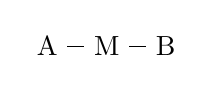
\begin{tikzpicture}
  \node (A) {A};
  \node[right=of A] (B) {B};
  \path (A) -- (B) node[midway] (M) {M};
  \draw (A) -- (M) -- (B);
\end{tikzpicture}
\begin{minipage}[c]{3cm}
  \begin{verbatim}
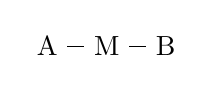
\begin{tikzpicture}
  \node (A) {A};
  \node[right=of A] (B) {B};
  \path (A) -- (B) node[midway] (M) {M};
  \draw (A) -- (M) -- (B);
\end{tikzpicture}
  \end{verbatim}
\end{minipage}\\

\textbf{Default distance between nodes}\\
\vspace{1ex}

\begin{tikzpicture}[node distance=0.2cm]
  \node (n1) {n1};
  \node[right=of n1] (n2) {n2};
\end{tikzpicture}
\begin{minipage}[c]{3cm}
  \begin{verbatim}

\begin{tikzpicture}[node distance=0.2cm]
  \node (n1) {n1};
  \node[right=of n1] (n2) {n2};
\end{tikzpicture}
  \end{verbatim}
\end{minipage}

\subsubsection{Absolute positioning on the page}
\begin{verbatim}
\begin{tikzpicture}[remember picture, overlay]
  \node [] (node1) at (current page.west) {};
\end{tikzpicture}
\end{verbatim}
% 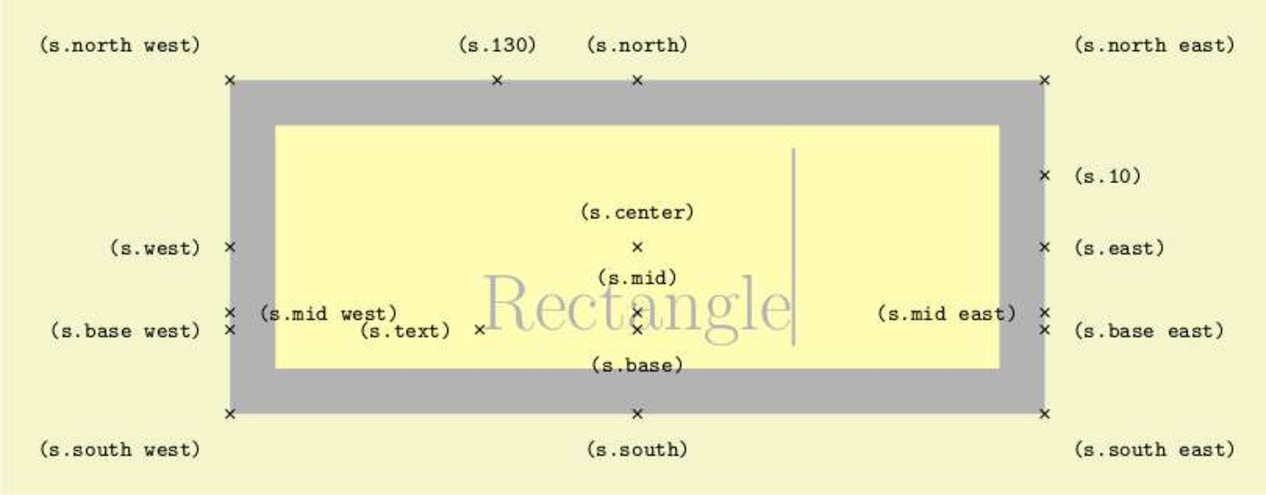
\includegraphics[width=0.33\textwidth]{figures/rectangle_shape.pdf}
\subsubsection{Matrix positioning}
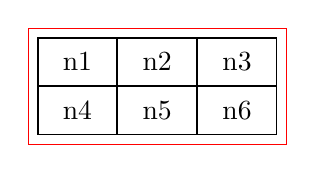
\begin{tikzpicture}
  [n/.style={draw,minimum width=1cm,minimum height=4ex,color=black}]
  \matrix[draw,color=red] (M) {
    \node[n] {n1}; &&
    \node[n] {n2}; &&
    \node[n] {n3}; \\
    \node[n] {n4}; &&
    \node[n] {n5}; &&
    \node[n] {n6}; \\
  };
\end{tikzpicture}
\begin{minipage}[c]{3cm}
  \begin{verbatim}
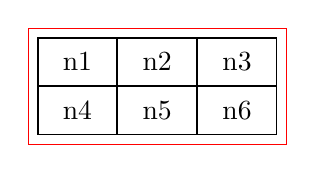
\begin{tikzpicture}
  [n/.style={draw,
             minimum width=1cm,
             minimum height=4ex,
             color=black}]
  \matrix[draw,color=red] (M) {
    \node[n] {n1}; &&
    \node[n] {n2}; &&
    \node[n] {n3}; \\
    \node[n] {n4}; &&
    \node[n] {n5}; &&
    \node[n] {n6}; \\
  };
\end{tikzpicture}
  \end{verbatim}
\end{minipage}

\subsection{Node dimension}
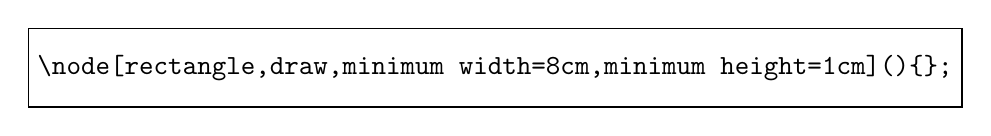
\begin{tikzpicture}
\node[rectangle,draw,minimum width=8cm, minimum height=1cm] () {\verb|\node[rectangle,draw,minimum width=8cm,minimum height=1cm](){};|};
\end{tikzpicture}

\subsection{Node shapes, filling colors and line width}

\begin{tikzpicture}
  \node[rectangle,draw=black,minimum width=1.5cm, minimum height=4ex] (rectangle) {}; 
  \node[right=0.2cm of rectangle]{\verb|\node[rectangle,draw=black](){};|};
\end{tikzpicture}

\begin{tikzpicture}
  \node[rectangle,draw=black,minimum width=1.5cm, minimum height=4ex,rounded corners] (rectangle) {}; 
  \node[right=0.2cm of rectangle]{\verb|\node[rectangle,draw=black,rounded corners](){};|};
\end{tikzpicture}

\begin{tikzpicture}
  \node[rectangle,draw=black,minimum width=1.5cm, minimum height=4ex,fill=blue] (rectangle) {}; 
  \node[right=0.2cm of rectangle]{\verb|\node[rectangle,draw=black,fill=blue](){};|};
\end{tikzpicture}

\begin{tikzpicture}
  \node[rectangle,draw=black,minimum width=1.5cm, minimum height=4ex, line width=2pt] (rectangle) {}; 
  \node[right=0.2cm of rectangle]{\verb|\node[rectangle,draw=black, line width=2pt](){};|};
\end{tikzpicture}

\subsection{Node options}
\subsubsection{Fonts and text colors}
\verb |node font=\tiny|\\
\verb |font=\bfseries| Node font in bold\\
\verb |text=blue| text color\\
\subsubsection{Text alignment in nodes}
\verb 'align=left|center|right' (handling carriage return in nodes)\\
\subsubsection{Style definition}
\verb |\begin{tikzpicture}[stylename/.style={node options...}]| Defining a node style named stylename\\
\verb |node[stylename] (node1) {};| Using a defined style\\

\vspace{1ex}
\textbf{Style definition for every node}\\
\begin{tikzpicture}[every node/.style={draw}]
  \node (n1) {n1};
  \node[right=of n1] (n2) {n2};
\end{tikzpicture}
\begin{minipage}[c]{3cm}
  \begin{verbatim}
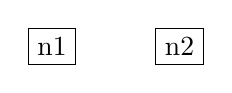
\begin{tikzpicture}[every node/.style={draw}]
  \node (n1) {n1};
  \node[right=of n1] (n2) {n2};
\end{tikzpicture}
  \end{verbatim}
\end{minipage}

\subsection{Arrows}
\begin{verbatim}
\coordinate (P1);
\coordinate[right=of P1] (P2);
\end{verbatim}
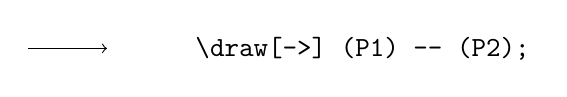
\begin{tikzpicture}
  \coordinate (P1);
  \coordinate[right=of P1] (P2);
  \draw[->] (P1) -- (P2);
  \node[right of=P2, anchor=west] {\verb|\draw[->] (P1) -- (P2);|};
\end{tikzpicture}
\begin{tikzpicture}
  \coordinate (P1);
  \coordinate[right=of P1] (P2);
  \draw[-Stealth] (P1) -- (P2);
  \node[right of=P2, anchor=west] {\verb|\draw[-Stealth] (P1) -- (P2);|};
\end{tikzpicture}
\begin{tikzpicture}
  \coordinate (P1);
  \coordinate[right=of P1] (P2);
  \draw[-{Stealth[round]}] (P1) -- (P2);
  \node[right of=P2, anchor=west] {\verb|\draw[-{Stealth[round]}] (P1) -- (P2);|};
\end{tikzpicture}
\begin{tikzpicture}
  \coordinate (P1);
  \coordinate[right=of P1] (P2);
  \draw[-{Stealth[round,length=4mm]}] (P1) -- (P2);
  \node[right of=P2, anchor=west] {\verb|\draw[-{Stealth[round,length=4mm]}] (P1) -- (P2);|};
\end{tikzpicture}
\verb |\begin{tikzpicture}[>={Stealth[round]}]| Defining an arrow style for the whole picture\\
\subsection{Node anchors}
\begin{adjustbox}{max totalsize={0.3\textwidth}{\textheight},center}
\begin{tikzpicture}[node distance = 1mm,
  shape example/.style = {
    color=black!50, draw, fill=blue!10,
    inner xsep=1.5cm, inner ysep=0.5cm,
}]
  \node[name=n,shape=rectangle,shape example]
    {\Huge rectan\smash{g}le\hspace{3cm}node};
  \foreach \anchor/\placement in
    {center/above, text/below, 45/above right,
       mid/right, mid east/right, mid west/left,
       base/below, base east/below right, base west/below left,
       north/above, south/below, east/above right, west/above left,
       north east/above, south east/below, south west/below, north west/above}
      \draw[shift=(n.\anchor)] plot[mark=x] coordinates{(0,0)}
        node[\placement,label distance = 0mm,inner sep=3pt]
          {\scriptsize\texttt{(n.\anchor)}};
\end{tikzpicture}
\end{adjustbox}
\begin{adjustbox}{max totalsize={0.3\textwidth}{\textheight},center}
\begin{tikzpicture}[font={\scriptsize\ttfamily}]
  \node[draw,rectangle,outer sep=1cm,inner sep=1cm,color=black!50, draw, fill=blue!10]
  (n) {{\sffamily\Large node n}};
  \draw[<->,thick,blue] (n.south)
      --++(0,1cm) node[midway,right]{outer sep};
  \draw[<->,thick,red] (n.south) ++(0,1cm) 
      --++(0,1cm)node[midway,right]{inner sep};
  \node[,outer sep=0,draw,left,color=black!50, draw, fill=blue!10,] 
      (m) at(n.west) {{\sffamily\Large node m}};
  \draw[<->,blue,thick] (m.east) -- ++(1cm,0) node[midway,above] {outer}
    node[midway,below] {sep};
  \draw[<->,red,thick] ($(n.west)+(1,0)$) -- ++(1cm,0) node[midway,above] {inner}
    node[midway,below] {sep};
  \foreach \anchor/\placement in
    {south west/below left,south/below,north/above,north west/above left,
       north east/above right,south east/below right}
       \draw[shift=(n.\anchor)] plot[mark=x] coordinates{(0,0)}
        node[\placement,label distance = 0mm,inner sep=3pt] {(n.\anchor)};
  \foreach \anchor/\placement in
    {west/left,south/below,north/above}
       \draw[shift=(m.\anchor)] plot[mark=x] coordinates{(0,0)}
        node[\placement,label distance = 0mm,inner sep=3pt] {(m.\anchor)};
  \draw[dashed] (n.south west) rectangle (n.north east);
  \node[above] at ($(n.center)!0.5!(n.north)$) {shape rectangle};
\end{tikzpicture}
\end{adjustbox}
Adapted from: \url{https://tikz.org/examples/chapter-03-drawing-positioning-and-aligning-nodes}

\subsection{Geometric figures}

\begin{tikzpicture}
  \draw[draw=black] (0,0) rectangle ++(2,1);
\end{tikzpicture}
\begin{minipage}[c]{3cm}
  \begin{verbatim}

\begin{tikzpicture}
  \draw[draw=black] (0,0) rectangle ++(2,1);
\end{tikzpicture}
\end{verbatim}
\end{minipage}\\

\begin{tikzpicture}
  \path[fill=lightgray] (0,0) rectangle ++(2,1);
\end{tikzpicture}
\begin{minipage}[c]{3cm}
  \begin{verbatim}

\begin{tikzpicture}
  \path[fill=lightgray] (0,0) rectangle ++(2,1);
\end{tikzpicture}
\end{verbatim}
\end{minipage}

\subsection{scope environment}
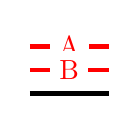
\begin{tikzpicture}[ultra thick]
  \begin{scope}[red]
    \draw (0mm,10mm) -- (10mm,10mm) 
      node[midway,fill=white] {A};
    \draw (0mm,7mm) -- (10mm,7mm)
      node[midway,fill=white] {B};
  \end{scope}
  \draw (0mm,4mm) -- (10mm,4mm);
\end{tikzpicture}
\begin{minipage}[c]{3cm}
  \begin{verbatim}
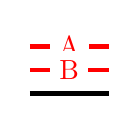
\begin{tikzpicture}[ultra thick]
  \begin{scope}[red]
    \draw (0mm,10mm) -- (10mm,10mm)
      node[midway,fill=white] {A};
    \draw (0mm,7mm) -- (10mm,7mm)
     node[midway,fill=white] {B};
  \end{scope}
  \draw (0mm,4mm) -- (10mm,4mm);
\end{tikzpicture}
  \end{verbatim}
\end{minipage}

\subsubsection{Positionning scopes relatively to other elements}
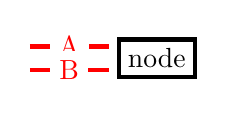
\begin{tikzpicture}[ultra thick]
  \begin{scope}[red,local bounding box=scope1]
    \draw (0mm,10mm) -- (10mm,10mm) 
      node[midway,fill=white] {A};
    \draw (0mm,7mm) -- (10mm,7mm)
      node[midway,fill=white] {B};
  \end{scope}
  \node[draw,right=0.1cm of scope1] {node};
\end{tikzpicture}
\begin{minipage}[c]{3cm}
  \begin{verbatim}
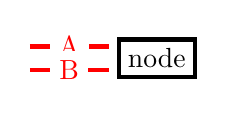
\begin{tikzpicture}[ultra thick]
  \begin{scope}[red,local bounding box=scope1]
    \draw (0mm,10mm) -- (10mm,10mm) 
      node[midway,fill=white] {A};
    \draw (0mm,7mm) -- (10mm,7mm)
      node[midway,fill=white] {B};
  \end{scope}
  \node[draw,right=0.1cm of scope1] {node};
\end{tikzpicture}
  \end{verbatim}
\end{minipage}

\begin{tikzpicture}[ultra thick]
  \node[draw] (node1) {node1};
  \begin{scope}[red,shift={($(node1.east)+(0.4cm,0)$)}]
    \node[draw] (A) {A};
    \node[draw,below=0.1cm of A] (B) {B};
  \end{scope}
\end{tikzpicture}
\begin{minipage}[c]{3cm}
  \begin{verbatim}
\begin{tikzpicture}[ultra thick]
  \node[draw] (node1) {node1};
  \begin{scope}[red,
          shift={($(node1.east)+(0.4cm,0)$)}]
    \node[draw] (A) {A};
    \node[draw,below=0.1cm of A] (B) {B};
  \end{scope}
\end{tikzpicture}
  \end{verbatim}
\end{minipage}

\subsection{Nested tikzpicture}
\begin{tikzpicture}[every node/.style={draw},
                    node distance=0.2cm]
  \node (n1) {n1};
  \node[right=of n1] (n2) {n2};
  \node[below=of n1] (n3) {n3};
  \node[below=of n2] (n4) {n4};
  \path (n2.east) -- (n4.east) coordinate[midway] (m);
  \node[right=of m] {
    \begin{tikzpicture}
      \node (n5) {n5}; 
      \node[right=of n5] (n6) {n6};
      \node[below=of n5] (n7) {n7};
      \node[below=of n6] (n8) {n8};
    \end{tikzpicture}
  };
\end{tikzpicture}
\begin{minipage}[c]{3cm}
  \begin{verbatim}
\begin{tikzpicture}[
    every node/.style={draw},
    node distance=0.2cm]
  \node (n1) {n1};
  \node[right=of n1] (n2) {n2};
  \node[below=of n1] (n3) {n3};
  \node[below=of n2] (n4) {n4};
  \path (n2.east) -- (n4.east)
    coordinate[midway] (m);
  \node[right=of m] {
    \begin{tikzpicture}
      \node (n5) {n5}; 
      \node[right=of n5] (n6) {n6};
      \node[below=of n5] (n7) {n7};
      \node[below=of n6] (n8) {n8};
    \end{tikzpicture}
  };
\end{tikzpicture}
  \end{verbatim}
\end{minipage}
